\newpage
\section{Introduction}
The purpose of this lab is to provide hands-on experience with a real MRI scanner to reinforce concepts covered in class. The system you will use is called OCRA: Open-source Console for Real-time Acquisition (Figure \ref{fig:ocra}).

OCRA came together from people all over the world: the MR Physics group at Harvard/MIT created an open-source tabletop scanner; visiting students at MGH translated the technology into a commercial product at the Research Campus STIMULATE of the Otto-von-Guericke University Magdeburg (Germany). Stanford now has three of these systems and we have worked on setting these up as educational tools for the suite of MRI courses offered by the departments of Electrical Engineering and Radiology.

This lab manual will begin by walking you through each component of the OCRA system followed by a brief overview of the basic functionality. Subsequent modules will guide you through exercises in using the scanner to probe a sample.

Take time to familiarize yourself with the components of this scanner. Throughout this lab you are encouraged to explore: if any experimental ideas come up beyond the lab directions, feel free to try these out and add the findings to your report (totally optional). This lab manual is a living document and your input WILL inspire future iterations.

\begin{figure}[h]
    \centering
    %\vspace{-8mm}
    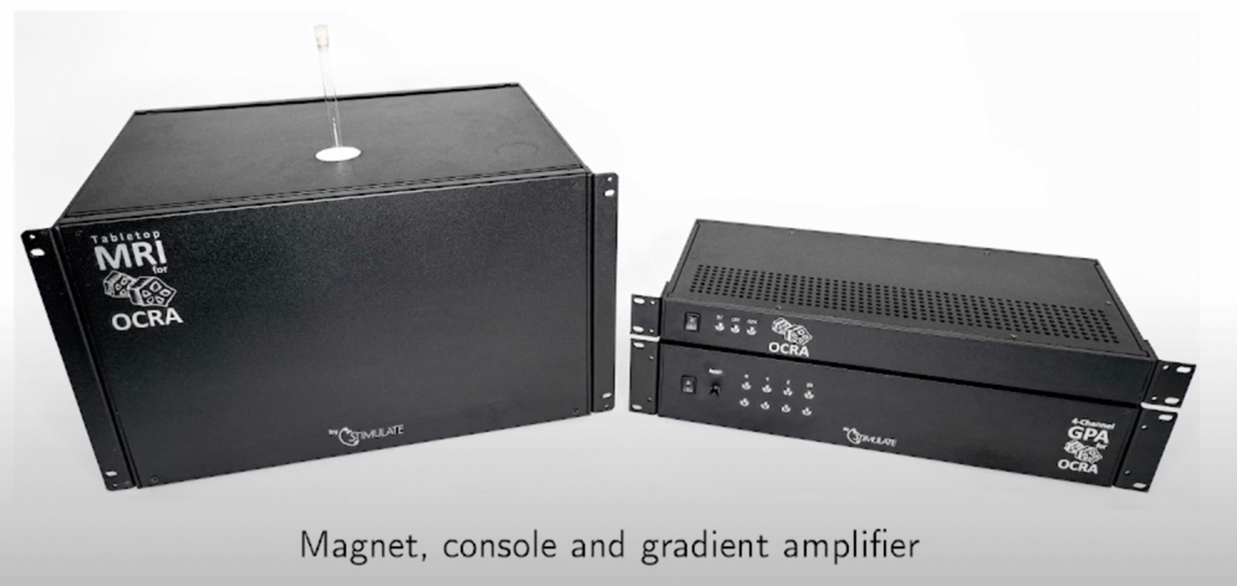
\includegraphics[width=0.9\textwidth]{ocra-system}
    \caption{\label{fig:ocra} OCRA tabletop MRI system including magnet box (left), console (top right) and gradient amplifier (bottom right).}
    \vspace{-5mm}
\end{figure}